\section{Introduction}\label{sec:intro}

Let $X$ be a smooth toric Fano variety of dimension $n$. We study slope
stability of its tangent bundle with respect to $H=-K_X$. The tangent
bundle of a nontrivial product is not stable. Connecting the factors by
a toric bundle or by invariant blowups can produce stability, but it can
also concentrate too much anticanonical degree in a proper tangent
subsheaf. This paper gives stability criteria and obstructions for two
classes of such connections, in unbounded dimension and Picard number.

For an invariant prime divisor $D_\rho$, write
\[
 \delta_\rho=\frac{nD_\rho H^{n-1}}{H^n}.
\]
These positive weights sum to $n$. The toric tangent-bundle criterion
says that stability is equivalent to
\[
 \sum_{u_\rho\in V}\delta_\rho<\dim V
\]
for every nonzero proper subspace spanned by primitive ray generators
\cite{Klyachko1990,HeringNillSuess2022}. Our first result reduces all
these inequalities to one divisor-degree inequality at each vertex of
a tree of blowups. We interpret the terms in that inequality as mixed
intersections on the exceptional centres. Our second result determines
a sharp Picard maximum for a class of toric bundles with arbitrary
integral twists. The maximum is attained by many different fans: every
fixed subcubic tree supplies extremizers after sufficiently long
independent subdivisions.

\subsection*{Blowup trees and exceptional intersections}
Let $G$ be a finite simple graph and choose integers $b_v\ge1$. Start
with $\prod_v\PP^{b_v}$ and assign distinct coordinate hyperplanes at
each factor to its incident edges. For each edge $\{v,w\}$, blow up
the codimension-two centre defined by its two assigned hyperplanes.
These star subdivisions commute. The resulting variety $Y(G,b)$ is
Fano exactly when $b_v\ge d_v:=\deg_G(v)$ for every $v$, and then
\[
 \dim Y(G,b)=\sum_v b_v,\qquad
 \rho(Y(G,b))=|V(G)|+|E(G)|.
\]
At each vertex there is an unassigned hyperplane. Its inverse image
has divisor class $D_v=f_v^*\mathcal O_{\PP^{b_v}}(1)$, where $f_v$
is the original factor projection composed with the blowdown. Set
$A_v=nD_vH^{n-1}/H^n$.

\begin{theorem}\label{thm:mixed-intro}
If $G$ is a tree with at least one edge and $b_v\ge d_v$ at every
vertex, then $T_{Y(G,b)}$ is anticanonically stable if and only if
$A_v<1$ for every $v$. It is semistable if and only if $A_v\le1$
for every $v$.
\end{theorem}

Theorem~\ref{mixed:tree} controls subspaces meeting arbitrarily many
factors, not just individual ray lines. At a nonleaf vertex with
$b_v=d_v$, the distinguished ray defines a rank-one foliation with
first Chern class $D_v$. Its degree satisfies the identity
\[
 (b_v+1)A_v=b_v+\sum_{e\ni v}J_{v,e}.
\]
Each $J_{v,e}$ is a positive first moment of the exceptional facet.
Section~\ref{sec:intrinsic} expresses it instead by ordinary mixed
intersections on the blowup centre, with the two normal directions
ordered by the factor projection. Moreover,
\[
 J_{v,e}+J_{w,e}=\frac{nE_eH^{n-1}}{H^n},\qquad
 \sum_{e\ni v}J_{v,e}
 =\frac{nf_v^*(-K_{\PP^{b_v}})H^{n-1}}{H^n}-b_v.
\]
Thus the number of incident blowups counts the contributions, but their
sizes and distribution determine whether the foliation violates stability.
The mixed-intersection formula applies to compatible blowup morphisms
without a tree hypothesis.

Call a vertex \emph{saturated} when $b_v=d_v$.
\begin{theorem}\label{thm:mixed-trees-intro}
Let $G$ be a tree with at least one edge and maximum degree at most
three. If every nonleaf vertex is saturated and the leaf dimensions
are arbitrary positive integers, then $T_{Y(G,b)}$ is anticanonically
stable. By contrast, a saturated degree-four vertex adjacent to four
saturated degree-four vertices forces instability, independently of
the farther branches of a Fano tree.
\end{theorem}

The assertions are Theorems~\ref{treemix:subcubic}
and~\ref{treemix:degree-four}. No separation or symmetry of the
branching vertices is required in the stable case. A saturated tree
with $M$ edges has dimension $2M$ and Picard number $2M+1$.
The degree bound three is sharp as a guarantee for every saturated
tree, but higher degree alone does not force instability. There are
stable trees with two branching vertices of degree four or five and
arbitrarily long connecting paths
(Proposition~\ref{treemix:two-centres}). The neighbouring dimensions
and the arrangement of branches enter the exceptional first moments.

\subsection*{A sharp bundle extremum and many extremizers}
Let $S_6$ denote the blowup of $\PP^2$ at its three torus-fixed points.
Consider locally trivial toric bundles with fibre $S_6^j$ over
$\prod_{c=1}^k\PP^{b_c}$, where $j,k,b_c\ge1$, in the fan
presentation~\eqref{interact:rays}. The twists are arbitrary integral
vectors in the fibre lattice.

\begin{theorem}\label{thm:main}\label{thm:bundlebound}
For every $n\ge4$, the largest Picard number among smooth toric Fano
$n$-folds in this bundle class with anticanonically stable tangent
bundle is
\[
 \left\lfloor\frac{5n}{4}\right\rfloor+1.
\]
\end{theorem}

The upper bound has three geometric sources. Fano positivity bounds
the number of nonzero twists at each base factor by its dimension.
A relative tangent slope obstruction requires each surface factor to
meet at least two base factors. Stability also excludes a disconnected
incidence graph. The resulting inequalities give the bound
(Theorem~\ref{interact:bound}). Paths of hexagon factors attain it in
dimension $4j$; end attachments give the other residue classes
(Corollary~\ref{attach:sharp}).

For a tree $\Gamma$, assign one hexagon factor to each edge and a base
$\PP^{\deg(v)}$ to each vertex. Twist the hexagon by opposite primitive
rays at its endpoints, as in Definition~\ref{graph:construction}, and
denote the bundle by $X(\Gamma)$.
\begin{theorem}\label{thm:tree-intro}
Every fixed finite tree of maximum degree three with at least one
edge gives stable $T_{X(\Gamma)}$ after replacing each edge by an
independently chosen sufficiently long path. A sufficient minimum
length depends only on the number $s$ of trivalent vertices and is
$O(\log s)$ as $s\to\infty$. If $\Gamma$ has $j$ edges, then
\[
 \dim X(\Gamma)=4j,\qquad \rho(X(\Gamma))=5j+1.
\]
For each integer $q\ge1$, every sufficiently large $j$ admits at least
$q$ pairwise nonisomorphic toric fans of such stable extremizers.
\end{theorem}

The subdivision assertion is Theorem~\ref{tree:stable}. Its abundance
consequence follows from recovering the graph from the fan
(Lemma~\ref{graph:reconstruction} and Corollary~\ref{tree:abundance}).
It concerns isomorphisms of toric fans. We do not claim a classification
of all extremizers. The exponential contraction of positive slice
functions explains the effect of separation, while a rank formula at
a cut controls subspaces extending across several branches.
Figure~\ref{fig:two-constructions} distinguishes this separation
phenomenon from the blowup theorem. Subdivision is not a general
stability-preserving operation: it can destabilize the blowup examples
(Corollary~\ref{branch:degree-five}).

\begin{figure}[tb]
\centering
\begin{adjustbox}{max width=\textwidth,center}
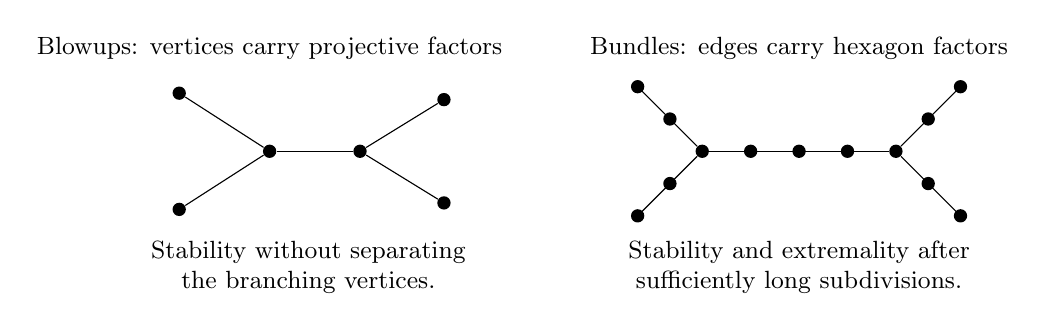
\begin{tikzpicture}[scale=.82,every node/.style={font=\small},
  vertex/.style={circle,fill=black,inner sep=1.7pt}]
\node[align=center] at (0,2.5) {Blowups: vertices carry projective factors};
\node[vertex] (a) at (0,0.9) {};
\foreach \name/\x/\y in {b/-1.4/1.8,c/-1.4/0,d/1.4/0.9}{
 \node[vertex] (\name) at (\x,\y) {}; \draw (a)--(\name);}
\foreach \name/\x/\y in {e/2.7/1.7,f/2.7/0.1}{
 \node[vertex] (\name) at (\x,\y) {}; \draw (d)--(\name);}
\node[align=center,text width=5.7cm] at (.6,-.9)
 {Stability without separating\\
 the branching vertices.};
\begin{scope}[xshift=8.2cm]
\node[align=center] at (0,2.5) {Bundles: edges carry hexagon factors};
\node[vertex] (p) at (-1.5,.9) {};
\node[vertex] (q) at (1.5,.9) {};
\foreach \x in {-.75,0,.75}{\node[vertex] at (\x,.9) {};}
\draw (p)--(q);
\foreach \x/\y in {-2.5/1.9,-2.5/-.1}{
 \draw (p)--(\x,\y);\node[vertex] at (\x,\y) {};
 \node[vertex] at ({(-1.5+\x)/2},{(.9+\y)/2}) {};}
\foreach \x/\y in {2.5/1.9,2.5/-.1}{
 \draw (q)--(\x,\y);\node[vertex] at (\x,\y) {};
 \node[vertex] at ({(1.5+\x)/2},{(.9+\y)/2}) {};}
\node[align=center,text width=5.7cm] at (0,-.9)
 {Stability and extremality after\\
 sufficiently long subdivisions.};
\end{scope}
\end{tikzpicture}
\end{adjustbox}
\caption{Two uses of a subcubic tree. On the left an edge specifies a
codimension-two blowup; on the right it specifies a fibre factor with
opposite twists. The right-hand subdivisions are schematic: the theorem
requires the stated sufficient lengths.}
\label{fig:two-constructions}
\end{figure}


\subsection*{Relation to earlier work and proof structure}
The subspace criterion and its interpretation as cone-volume
concentration are established toric stability theory
\cite{Klyachko1990,HeringNillSuess2022}. Hering--Nill--S\"u\ss{}
determine stability regions for smooth toric surfaces and varieties
of Picard rank two. Dasgupta--Dey--Khan independently treat Picard
rank two and classify the smooth toric Fano fourfolds of Picard rank
three \cite{DasguptaDeyKhan2020}; the Picard-rank-at-most-two
fourfold case is due to Biswas--Dey--Genc--Poddar
\cite{BiswasDeyGencPoddar2021}. Reynolds treats all $124$ smooth toric
Fano fourfolds and their unstable Harder--Narasimhan filtrations
\cite{Reynolds2023}. Devey develops finite matroid tests for
equivariant reflexive sheaves \cite{Devey2022}. We use saturated
subsheaves, as required by the erratum \cite{DasguptaDeyKhan2021}.
The single-edge blowup with dimensions $(1,3)$ is already stable by
\cite[Proposition~5.6.1(2)]{DasguptaDeyKhan2020}.

Our results address families with no bound on the dimension or number
of factors. For blowups, the new steps are the tree reduction, the
exceptional mixed-intersection identity, and uniform estimates that
separate stable from destabilizing arrangements. The estimates use
Efron's monotonicity theorem through
\cite[Theorems~3.2--3.3]{saumardwellner2018}.
For bundles, the relative tangent obstruction uses a divergence
identity related to \cite[Lemma~2.2 and Eq.~(4.4)]{HenkLinke2014}.
Unlike a centred unweighted fibre polytope, its density weighted by
base-slice volumes may have nonzero first moment. This distinction
gives the obstruction. The polarization is the fixed divisor $-K_X$;
results for polarizations near a pulled-back or contracted class
\cite{NapameTipler2024,ClarkeNapameTipler2025} do not give the needed
inequalities. The preceding paper \cite{Wuebben2026} constructs stable
root-twisted bundles with $\rho=n+2$; allowing the number of surface
factors to grow produces the larger extremum and branching families here.

The bundle existence proofs combine exact finite rational inequalities
with the Birkhoff--Hopf contraction theorem
\cite{EvesonNussbaum1995} and induction. The finite calculations are
premises of proofs covering all lengths, not numerical extrapolations.
Their matrices, inequalities and error estimates are printed in the
appendices and reproduced by the ancillary code. The blowup-tree
arguments use uniform identities, integral comparisons and induction,
with explicit polynomial arithmetic. Appendix~\ref{sec:computation}
also records completed classification checks, including the unique
stable eightfold of Picard number eleven.

After the common stability criterion, Sections~\ref{sec:mixed}--\ref{sec:mixed-tree-threshold}
develop the blowup results. Sections~\ref{sec:interactions}--\ref{sec:subdivided}
treat the bundle obstruction, sharpness and abundance. Complete
path, attachment and three-arm calculations, followed by secondary
families and classification data, are in the appendices. Both Picard
maxima concern specified constructions. The unrestricted extremum
remains open and is discussed in Section~\ref{sec:questions}.
